\documentclass[review]{elsarticle}
\usepackage{hyperref}
\usepackage[margin=1in]{geometry}
\usepackage{graphicx}
\usepackage{amsmath}
\usepackage{placeins}
\usepackage{comment}
\usepackage{gensymb}
\usepackage{lineno}
\usepackage{flexisym}
\usepackage{color}

\journal{Journal of Nuclear Materials}
\bibliographystyle{elsarticle-num}

\begin{document}

\begin{frontmatter}
\title{\textit{Ab initio} molecular dynamics investigation of $\gamma$-U}

\author[inl]{Benjamin Beeler\corref{qwe}}
\cortext[qwe]{Corresponding author}
\ead{benjamin.beeler@inl.gov}
\author[lanl]{David Andersson}
\author[inl]{Chao Jiang}
\author[inl]{Yongfeng Zhang}
\address[inl]{Idaho National Laboratory, Idaho Falls, ID 83415}
\address[lanl]{Los Alamos National Laboratory, Los Alamos, NM 87545}

\begin{abstract}

Uranium (U) is often alloyed with molybdenum (Mo) or zirconium (Zr) in order to stabilize the high-temperature body-centered cubic $\gamma$ phase of uranium for use in nuclear reactors. However, relatively little experimental or computational investigation has centered on $\gamma$-U, largely due to the mechanical instability of this phase at room temperature. This is particularly problematic for density functional theory calculations that typically investigate 0 K properties. However, \textit{ab initio} molecular dynamics (AIMD) allows for quantum mechanical-based calculations to be performed at non-zero temperatures. In this work, AIMD simulations are performed to calculate the equilibrium volume for the $\gamma$ phase of U from 800 K to 1400 K. Utilizing the volume at each temperature, the bulk modulus, the radial distribution function, the interstitial and vacancy formation energies, and the diffusion coefficients are determined. This is the first AIMD investigation of point defects in $\gamma$-U. 

\end{abstract}
\end{frontmatter}

\section{Introduction}

Uranium (U) is an actinide exhibiting delocalized f-electrons that exists in three solid phases: $\alpha$ (face-centered orthorhombic), $\beta$ (body-centered tetragonal) and $\gamma$ (body-centered cubic) \cite{yoo1998}. At elevated temperatures, U transforms from $\alpha$ to $\beta$ at approximately 935 K and $\beta$ transforms to $\gamma$ at approximately 1045 K \cite{soderlind1998}. Uranium is alloyed with Mo or Zr in order to stabilize the preferred body-centered cubic phase to lower temperatures, most notably for application as nuclear fuel. 

Density functional theory (DFT) is an essential part of computational materials science, addressing a variety of problems in materials design and processing on a fundamental level. Several examinations of U via DFT have been performed on the orthorhombic and body-centered cubic (bcc) structures of U. Taylor \cite{taylor2008} used a projector augmented wave (PAW) pseudopotential to calculate the lattice constants of $\alpha$-U and $\gamma$-U along with the bulk modulus of both phases. Xiang, \textit{et al.} \cite{xiang2008} also utilized a PAW pseudopotential to perform an analysis of bulk properties in the $\alpha$ and $\gamma$ phases, as well as an analysis of defects in $\gamma$-U.  Beeler, \textit{et al.} calculated the lattice constants and elastic constants of $\alpha$, $\beta$ and $\gamma$-U \cite{beeler2013}, in addition to the point defect properties in both $\alpha$ and $\gamma$-U \cite{beeler2010}. Huang and Wirth \cite{wirth2011, wirth2012} calculated intrinsic and extrinsic point defect formation energies and migration barriers in $\alpha$-U. These DFT investigations showed a general, if imperfect, agreement with the experimental bulk moduli, lattice and elastic constants and vacancy formation energy \cite{yoo1998, barrett1963, matter1980}. 

The explanation for such a limited scope of analysis on the $\gamma$ phase lies partially in the inherent issues associated with a DFT approach to the study of a high temperature phase. DFT calculations are typically performed to calculate ground state properties, implying that the calculation is taking place at a temperature equal to 0 K. It has been shown, via the calculation of elastic constants, that the elastic shear constant (C\textprime=$\frac{1}{2}$(C$_{11}$-C$_{12}$)) is negative in the body-centered cubic phase of U \cite{soderlind1998, beeler2013}. Thus, at low temperatures $\gamma$-U is mechanically unstable. Computationally, this mechanical instability translates into an inability to calculate relaxed structures involving defects, due to the inherent localized deformation created by introducing a point defect that leads to deconstruction of the crystal lattice. Several other systems, such as Zr, Ti, and Hf, also exhibit a high temperature bcc phase that is mechanically unstable at low temperature \cite{sanchez1975, ye1987}. Beeler, \textit{et al.} \cite{beeler2010} attempted to circumvent this mechanical instability via the introduction of a ``shell" relaxation scheme, in which only a select group of atoms was permitted to relax around the defect. This methodology can provide an approximation for defect energies, but the accuracy of such a tactic is unclear. Additionally, this only provides an approximation for defect energies at 0 K and provides no insight into defect energetics at elevated temperatures and the extrapolation of properties at 0 K to high temperature systems is inexact at best.  

\textit{Ab initio} molecular dynamics (AIMD) allows for quantum mechanical-based calculations to be performed at non-zero temperatures. AIMD can account for the inherent anharmonicity responsible for making the bcc phase stable at high temperature, and as such allows for direct investigation of the bcc phase without any other required assumptions or restrictions.  AIMD has been utilized to study a variety of systems including liquid phase diffusion in Al-Si \cite{manga2018}, adsorption energy of Fe on TiN surfaces \cite{wang2010}, NaCl dissolution in water \cite{timko2010} and finite temperature phonon dispersion curves in bcc Zr and bcc Li \cite{hellman2011}. Hood, \textit{et al.} \cite{hood2008} have previously utilized AIMD to study the equation of state of U and the variation in density of states for the liquid phase of U at two unique temperatures. Hood, \textit{et al.} utilized a unique pseudopotential that was presented in that same manuscript \cite{hood2008}. Soderlind, \textit{et al.} \cite{soderlind2012} utilized self-consistent \textit{ab initio} lattice dynamics (SCAILD) to study the high temperature stabilization of the $\gamma$-U phase by calculating phonon modes at 1100 K. There have been no investigations in the free energy via the temperature dependent effect potential (TDEP) technique \cite{hellman2013} nor any AIMD investigations into the defect formation energies in $\gamma$-U at high temperatures. 

In this work, AIMD simulations are performed to calculate the energy as a function of volume for the $\gamma$ phase of U from 800 K to 1400 K. Utilizing the equilibrium volume at each temperature, the bulk modulus, the radial distribution function, the interstitial and vacancy formation energies, and the diffusion coefficients are determined. This is the first AIMD investigation of point defects in $\gamma$-U. 

\section{Computational Details}
Systems are investigated using the Vienna \textit{ab initio} Simulation Package (VASP) \cite{vasp1, vasp2, vasp3, vasp4}. The projector augmented wave (PAW) method \cite{paw1, paw2} is utilized within the density functional theory \cite{dft1, dft2} framework. Calculations are performed using the Perdew-Burke-Ernzerhof (PBE) \cite{pbe1, pbe2} generalized gradient approximation (GGA) density functional implementation for the description of the exchange-correlation. An uranium PAW pseudopotential with the 6s$^{2}$6p$^{6}$5f$^{3}$6d$^{1}$7s$^{2}$ valence electronic configuration and a core represented by [Xe, 5d, 4f] is utilized. Methfessel and Paxton's smearing method \cite{methfessel} of the first order is used with a width of 0.2 eV to determine the partial occupancies for each wavefunction. A Monkhorst-Pack \cite{monkhorst} 2x2x2 k-point mesh was utilized for Brillouin zone sampling. Uranium is assumed to be non-magnetic, in accordance with both experiments and previous simulations, and as such calculations are non spin polarized. The precision is set to accurate and the energy cutoff is increased to 500 eV. The electronic self-consistent loop exit criterion is set to 10$^{-4}$.  A 54 atom supercell (3x3x3) is utilized for all simulations. Dynamics were carried out in the NVT ensemble with a Nose-Hoover thermostat to control temperature, calculating both the forces and the stress tensor. The Nose mass was set to 0, allowing a period of 40 time steps. The timestep is set to 5 fs, and the simulation is carried out for 2000 timesteps (10 ps). In order to obtain average properties over the \textit{ab initio} molecular dynamics simulation, the energies and pressures for the final 1000 timesteps are extracted and averaged. The trajectories of the total supercell energy and pressure as a function of time step for an example simulation are shown in Fig. \ref{fig:convergence}. The energy and pressure both converge relatively quickly to a given value, with the energy oscillating by approximately $\pm$ 2 eV while the pressure oscillates by approximately $\pm$ 15 kB throughout the simulation. Additionally, five unique simulations are performed with different random seeds in order to ensure statistical significance of the results. The system is verified to remain bcc by averaging the positions of the atoms over the final 1000 timesteps and performing a common neighbor analysis with the Ovito \cite{ovito} visualization software. 

\begin{figure}[h]
 \centering
 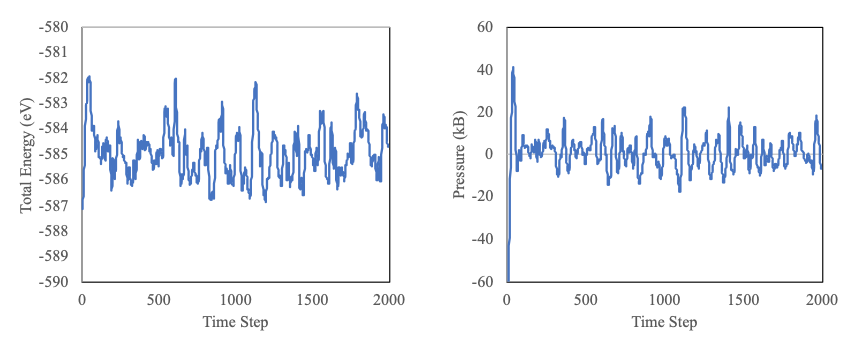
\includegraphics[width=0.95\textwidth]{convergence.png} 
 \caption{An example total supercell energy and pressure as a function of time. Data is extracted and averaged over the final 1000 timesteps to determine an energy and pressure for a given system. }
 \label{fig:convergence}
\end{figure}

\FloatBarrier

The system was evaluated at a series of volumes in order to construct a pressure as a function of volume (P(V)) relationship. The lattice constant is varied from 3.47 {\AA} up to 3.52 {\AA} in increments of 0.01 {\AA}. The point at which the P(V) relationship is equal to zero is determined to be the equilibrium volume. The energy is additionally determined at the determined equilibrium volume. A second order polynomial function is fit to the dataset. The P(V) curve was constructed for temperatures from 800 K up to 1400 K, in increments of 100 K. The melting point of uranium is 1408 K and the phase transition temperature into the $\gamma$ phase is 1045 K, thus this set of temperatures spans the entire range of stability for the $\gamma$ phase as well as exploring lower temperatures where the $\gamma$ phase is stable, but not the equilibrium structure. The bulk modulus can be determined by taking the first derivative of pressure versus volume relationship with respect to volume:

\begin{equation}
\label{eq:bulk}
B_{0} = -V_0 \left( \frac{\partial P}{\partial V} \right)
\end{equation}

where B$_0$ is the bulk modulus, V$_0$ is the equilibrium volume and P is the pressure. Thus, the second order Birch-Murnaghan equation of state (EOS) in equation \ref{eq:eos} can be parametrized to the pressure as a function of volume using the calculated data. 

\begin{equation}
\label{eq:eos}
P(V) = \frac{3B_0}{2} \left[ \left(\frac{V_0}{V}\right)^{\frac{7}{3}} - \left(\frac{V_0}{V}\right)^{\frac{5}{3}} \right]
\end{equation}


The formation energy of point defects is calculated via equation \ref{eq:eform}: 

\begin{equation}
\label{eq:eform}
E_f = E^* - \frac{n \pm 1}{n} \times E_0
\end{equation}

where E$^{*}$ is the energy of a system with a defect (with n $\pm 1$ atoms), \textit{n} is the number of atoms in the defect-free system and E$_{0}$ is the energy of a defect-free system with \textit{n} atoms. Equation \ref{eq:eform} utilizes (\textit{n} + 1) for interstitials and (\textit{n} - 1) for vacancies. All defect properties are determined in constant volume systems, set to the equilibrium volume for a given temperature. 

The diffusion coefficients for individual point defects and for self-diffusion in $\gamma$-U were determined by calculation of the mean-squared displacement ($\langle$r$^2$$\rangle$) of atoms. The magnitude of $\langle$r$^2$$\rangle$ was determined via scripts from the VTST webpage \cite{vtst}. The $\langle$r$^2$$\rangle$ value for random atomic motion in a defect-free system is subtracted from the total $\langle$r$^2$$\rangle$ in order to ensure only displacements from the individual point defects are included. The diffusion coefficient is determined from the Einstein formula (D=$\langle$r$^2$$\rangle$/6t), where \textit{t} is the time. Systems are evolved for 100 ps, in increments of 5 ps, to obtain the $\langle$r$^2$$\rangle$ as a function of time. Given that these simulations are so computationally expensive, only a single representative system is used for each temperature and defect type. Thus, this data is only proposed to be an informative estimate of the diffusion of point defects in $\gamma$-U. 

The computational expense associated with these kinds of investigations should be emphasized. Over one million cpu-hours on a high-performance computing system were required to obtain the data within this manuscript, not including scoping and convergence testing. Ideally, both larger systems would be analyzed and additional simulations would be performed to increase the statistical accuracy of the results. However, the accuracy was deemed sufficient to provide meaningful results (as will be shown), taking into account the computational expense associated with increasing statistical significance. 

\section{Results}
\subsection{Bulk Modulus of $\gamma$-U}

The pressure as a function of volume for $\gamma$-U from 800 K to 1400 K is shown in Fig. \ref{fig:pvsv}, with the fit second-order Birch-Murnaghan equation of state (EOS) for each temperature. The equilibrium volume is taken as the zero-crossing of each curve at a given temperature. It can be observed that volumetric expansion takes place over this temperature range. Both Touloukian \cite{touloukian} and Basak \cite{basak} experimentally determined thermal expansion for $\gamma$-U and produced an empirical fit as a function of temperature, which translates to a linear thermal expansion (LTE) coefficient. The data from Touloukian leads to a LTE of 22.4 x 10$^{-6}$ K$^{-1}$ and the work of Basak lead to a LTE of 13.3 x 10$^{-6}$ K$^{-1}$, although the data from Basak is over a smaller temperature range. A comparison of the data calculated in this work to the experimental data is shown in Fig. \ref{fig:exp}. The thermal expansion is taken with respect to a system at 1100 K in order to compare with the experimental data, thus the expansion at 1100 K is zero. The AIMD simulations under-predict the thermal expansion compared to Touloukian, while exactly matching the values of Basak on the limited temperature range of 1100 - 1200 K. When including the entire temperature range from the AIMD calculations, the calculated of the LTE of 11.3 x 10$^{-6}$ K$^{-1}$, underestimating both experimental values.

The lattice constant is also underestimated when compared to experiment. At 1060 K, Lawson \cite{lawson1988} found the lattice constant to be 3.53 {\AA}, while this work predicts 3.501 {\AA}. Previous DFT work has shown that the lattice constant of $\gamma$-U is underestimated compared to experimental values, however when those experimental values extrapolated to 0 K, the results shown an overprediction of the lattice constant\cite{beeler2010, xie2013}. Utilizing a Hubbard U parameter within DFT has been shown to increase the lattice constant of $\gamma$-U \cite{xie2013}, and as such it is possible that AIMD with the inclusion of the Hubbard U parameter would yield equilibrium volumes that more closely match the experimental values, although this is not a sufficient argument to use the Hubbard U parameter. It is unclear what the effect of the Hubbard U parameter would be on other properties of interest. 

\begin{figure}[h]
 \centering
 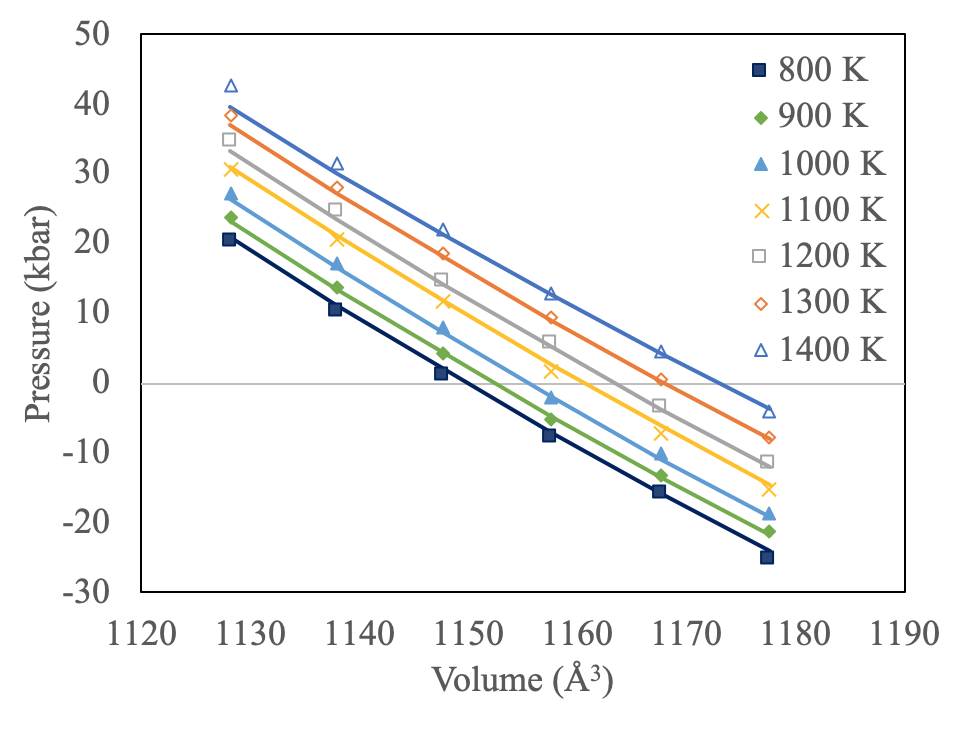
\includegraphics[width=0.75\textwidth]{p_vs_v.png} 
 \caption{The energy per atom as a function of volume for $\gamma$-U from 800 K to 1400 K. Lines are the second-order Birch-Murnaghan equation of state (EOS) fits to the data.   }
 \label{fig:pvsv}
\end{figure}

\begin{figure}[h]
 \centering
 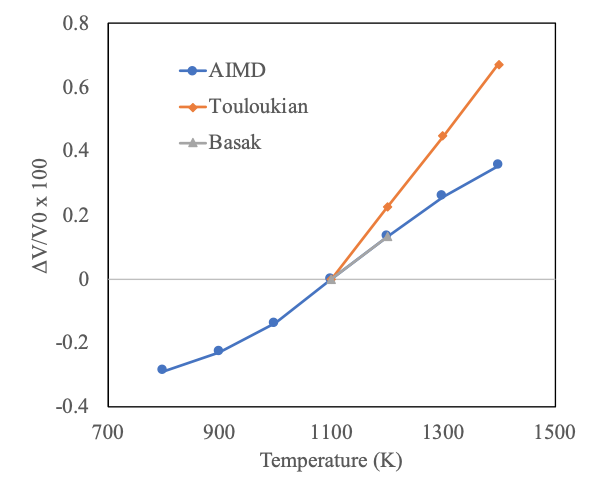
\includegraphics[width=0.75\textwidth]{thermal_exp.png} 
 \caption{The thermal expansion with respect to a system at 1100 K for this work (AIMD) and experimental work from Touloukian \cite{touloukian} and Basak \cite{basak} .   }
 \label{fig:exp}
\end{figure}

\FloatBarrier

The bulk modulus calculated from equation \ref{eq:bulk} is shown in Table \ref{tab:bulk}. There is a general softening of the bulk modulus with increasing temperature, as would be expected. The softening is exacerbated moving from 1300 K to 1400 K, likely due to the proximity to the melting point. An experimental value of the bulk modulus was calculated by Yoo \cite{yoo1998} as 113 GPa, utilizing a temperature independent equation of state. The values in this work are only slightly lower than the experimental work (by approximately 7 {\%}). This provides additional confidence in this methodology. 

\begin{table}[h]
\caption{The bulk modulus of $\gamma$-U from 800 K to 1400 K.} \label{tab:bulk}
\begin{center}
\begin{tabular}{|c|c|}
	\hline
	Temperature (K) & Bulk Modulus (GPa) \\
	 \hline
	 800 & 106.1 \\
	 900 & 105.6 \\
	 1000 & 105.9 \\
	 1100 & 104.7 \\
	 1200 & 101.2 \\	 
	 1300 & 99.0 \\
	 1400 & 94.7 \\
	 \hline
\end{tabular}
\end{center}
\label{default}
\end{table}

\FloatBarrier

The radial distribution function (rdf or g(r)) is calculated at the equilibrium volume for each temperature and is displayed in Fig. \ref{fig:rdf}. The ideal bcc structure with a lattice parameter of 3.51 {\AA} is included for reference on a secondary axis. The rdf is determined from the average positions of the atoms in a given simulation over the final 1000 timesteps. It is clear from Fig. \ref{fig:rdf} that the bcc structure is present for all temperatures, as the peak locations are exactly matched for all temperatures. However, at the low temperature regime near 800 K, additional peak roughening or broadening is observed, particularly for 1st, 3rd and 4th nearest neighbor peaks. This is exactly the opposite behavior of what would be expected, in that given the same crystal structure, the peaks should be narrower at lower temperatures and broader at higher temperatures. Thus it is expected that 800 K is near the stability transition for the bcc structure of U and we are witnessing slight distortions away from the perfect bcc crystal structure. As such, the rest of the manuscript will exclude examinations at 800 K.

\begin{figure}[h]
 \centering
 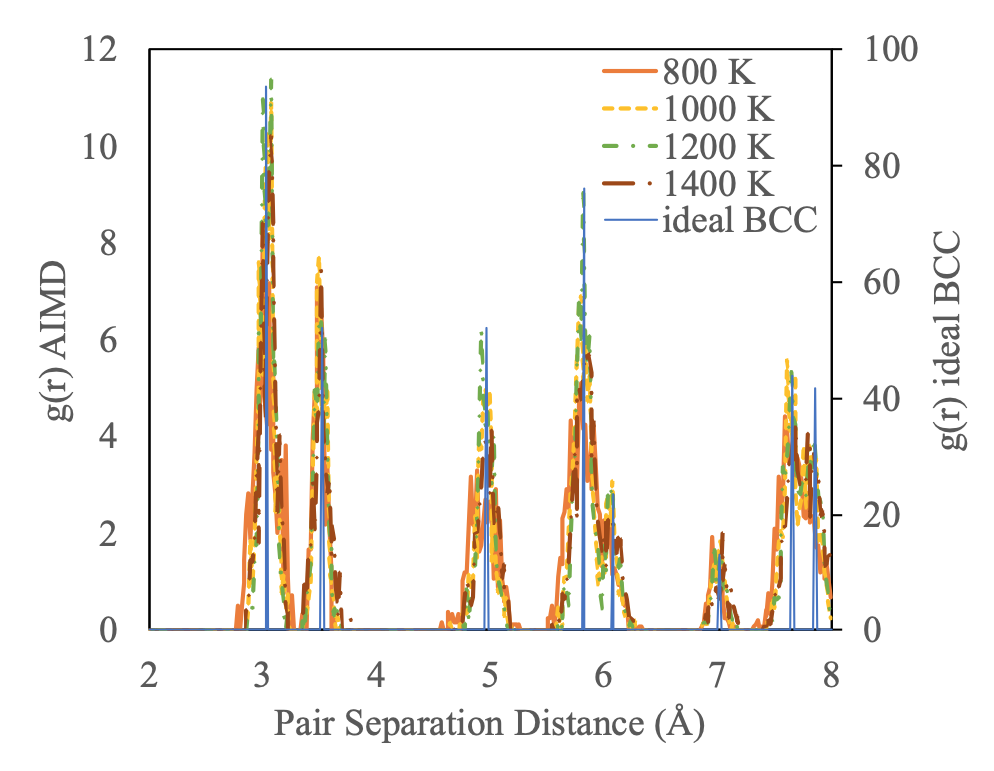
\includegraphics[width=0.8\textwidth]{rdf_final.png} 
 \caption{The radial distribution function (g(r)) for $\gamma$-U from 800 K to 1400 K. The ideal bcc structure with a lattice parameter of 3.51 {\AA} is included for reference on a secondary axis.  }
 \label{fig:rdf}
\end{figure}

\FloatBarrier

\subsection{Point Defect Energies of $\gamma$-U}

The point defect formation energy as a function of temperature is shown in Fig. \ref{fig:eform}. Data for both interstitials and vacancies is shown, with error bars representing plus/minus twice the standard error of the data set (95\% confidence interval). The standard error for the formation energy is the sum of the standard error of the energy for a system with a point defect (E$^*$ in equation \ref{eq:eform}) and the standard error of the energy of a system with no defects (E$_0$ from equation \ref{eq:eform}). The data in Fig. \ref{fig:eform} is also presented in Table \ref{tab:defs}. Data at 800 K is excluded from this analysis, as it was shown in Fig. \ref{fig:rdf} that this system is approaching the stability transition and thus could potentially exhibit anomalous effects. 

The first thing to note is that the interstitial formation energy is substantially lower than the vacancy formation energy across the entire temperature regime investigated. This is not the case in $\alpha$-U \cite{wirth2011} or in most metals \cite{schultz1968, baskes1979, lee2001, lee2003}, where the interstitial formation energy is substantially higher than the vacancy formation energy. However, this is in agreement with previous computational results \cite{beeler2010} as well as the experimental evidence suggesting that self-diffusion in $\gamma$-U is at least partially due to an interstitialcy mechanism \cite{fedorov1978, smirnov1992, mehrer2011}. The positron annihilation experimental investigations that have studied the vacancy formation energy in $\gamma$-U correspond with the magnitude of the vacancy formation energies from this work. Matter \cite{matter1980} reported a vacancy formation energy of 1.2$\pm$0.25 eV, while Lund \cite{lund2013} reported a value of 1.6$\pm$0.2 eV, although Lund suggested that oxygen impurities likely affected their results. There are no experimental results of interstitial formation energy for comparison.

The formation energy of both vacancies and interstitials increases with increasing temperature. This variance in vacancy formation energy has been previously shown in Al by Carling \cite{carling2003} and in Fe and Zr by Mendelev \cite{mendelev2009, mendelev2010}. Mendelev also saw an increase in the interstitial formation energy with increasing temperature in Zr \cite{mendelev2010}. Defect behavior in U has been compared to Zr due to the hexagonal-type ground state structures for both elements paired with high temperature bcc structures, in addition to similar anomalous diffusive behavior \cite{matter1980,kidson1961}. The magnitude of increase (0.5 - 1 eV) observed in this work is in line with these previous studies. The variation in the ratio of the vacancy formation energy to the interstitial formation energy decreases slightly with increasing temperature.

The magnitude of the formation energies, particularly for interstitials, should be emphasized. This work compares very favorably to the previous DFT study on point defects in $\gamma$-U at 0 K\cite{beeler2010}, which showed the interstitial formation energy as low as 0.5 eV. Despite this agreement, the formation energies seem abnormally low.  Neglecting entropic effects, the formation energies at the provided temperatures would yield equilibrium interstitial concentrations on the order of 10$^{-3}$ defects per atom. Additionally, the inclusion of entropic effects should \textit{increase} the equilibrium defect concentrations. Typically such high defect concentrations are not observed except for very close to the melting point. However, this work suggests such defect concentrations across the entire temperature range of phase stability for the $\gamma$ phase (0.64T$_m$ - 1.0T$_m$). It has been shown that increasing defect concentration leads to a decrease in melting point \cite{sorkin2003}, and it is possible that the low interstitial formation energy in $\gamma$-U leads to the comparatively low melting of U compared to Zr or other bcc metals \cite{williams1990} such as Fe, V or Mo, which all have higher interstitial formation energies \cite{mendelev2010, mendelev2009, nguyen2006} as well as higher melting points. Other possibilities include that entropic effects play an important role in determining the equilibrium defect concentrations or investigating point defects in the dilute approximation has limited applicability in $\gamma$-U. It is regretfully beyond the scope of this work, and debatably beyond the scope of current computational capabilities, to thoroughly examine defect clusters in $\gamma$-U in an AIMD framework and obtain statistical significance. 

\begin{comment}
\textit{at these point defect energies, and neglecting entropic effects (which is clearly necessary), the point defect concentrations actually decrease with increasing temperature. so... entropy must play an important role in determining point defect concentrations. or there is an athermal point defect concentration that is predicted. }

\textit{also, my numbers are 1200 K are a jump in the data. seems something might be slightly off equilibrium here...}
\end{comment}

 \begin{figure}[h]
 \centering
 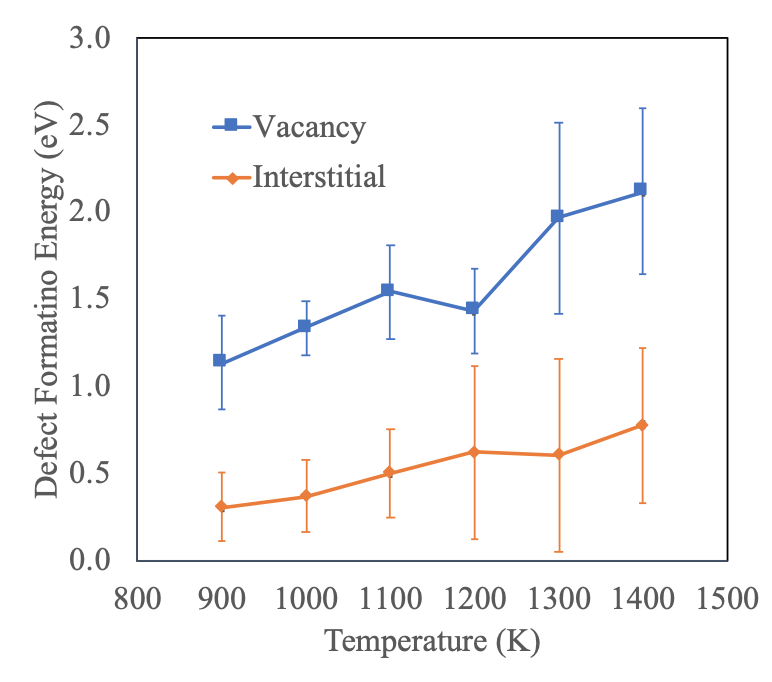
\includegraphics[width=0.75\textwidth]{eform.png} 
 \caption{The point defect formation energy for $\gamma$-U from 900 K to 1400 K. Error bars represent plus/minus one standard error of the data set. }
 \label{fig:eform}
\end{figure}

\begin{table}[h]
\caption{The point defect formation energy for vacancies (E$_{f}^{v}$) and interstitials (E$_{f}^{i}$) in $\gamma$-U from 900 K to 1400 K.} \label{tab:defs}
\begin{center}
\begin{tabular}{|c|c|c|}
	\hline
	Temperature (K) & E$_{f}^{v}$ (eV) & E$_{f}^{i}$ (eV) \\
	 \hline
  	   900 & 1.14 & 0.31 \\
	 1000 & 1.34 & 0.37 \\
	 1100 & 1.54 & 0.50 \\
	 1200 & 1.43 & 0.62 \\
	 1300 & 1.97 & 0.61 \\
	 1400 & 2.12 & 0.78 \\
	 \hline
\end{tabular}
\end{center}
\label{default}
\end{table}

\FloatBarrier

\subsection{Point Defect Diffusion in $\gamma$-U}

The mean squared displacement ($\langle$r$^2$$\rangle$) as a function of time was tracked over 100 ps for systems with an individual point defect. The $\langle$r$^2$$\rangle$ data for interstitials and vacancies is shown in Fig. \ref{fig:rsquare}. Given that only one individual system is utilized and that only a relatively short period of time is investigated, there is inherently substantial statistical fluctuation in the data. In spite of this, the $\langle$r$^2$$\rangle$ behavior is generally linear with time and diffusion coefficients can be estimated. A slight decrease in the $\langle$r$^2$$\rangle$ value can be observed for vacancies moving from 1200 K to 1300 K. This is likely an artifact of small sample size in a system with strong thermal fluctuations and should not be interpreted as actually indicating reduced diffusion at higher temperature. The calculated diffusion coefficients for vacancies and interstitials are shown in Fig. \ref{fig:diff}. It can be seen that the diffusion coefficient for interstitials and vacancies exhibits a similar magnitude, albeit unique slopes. Interestingly, this study shows that the vacancy displays a lower migration barrier than the interstitial. The vacancy diffusion coefficient is higher in the low temperature regime (1000K-1100K) while the interstitial diffusion coefficient is higher in the high temperature regime (1200K-1300K).  An exponential function can be fit to the data to obtain a pre-factor and a migration barrier for each point defect. This data is reported in Table \ref{tab:diff}. 

 \begin{figure}[h]
 \centering
 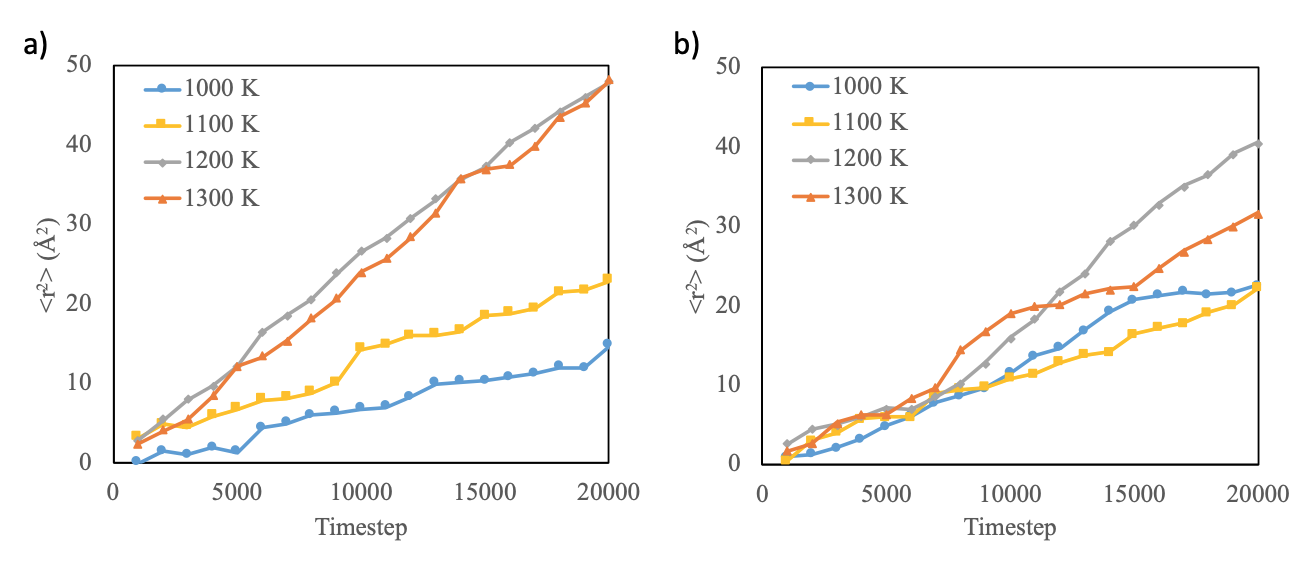
\includegraphics[width=0.9\textwidth]{msd.png} 
 \caption{The mean-squared displacement as a function of time for a) interstitials and b) vacancies from 1000 K to 1400 K.  }
 \label{fig:rsquare}
\end{figure}

 \begin{figure}[h]
 \centering
 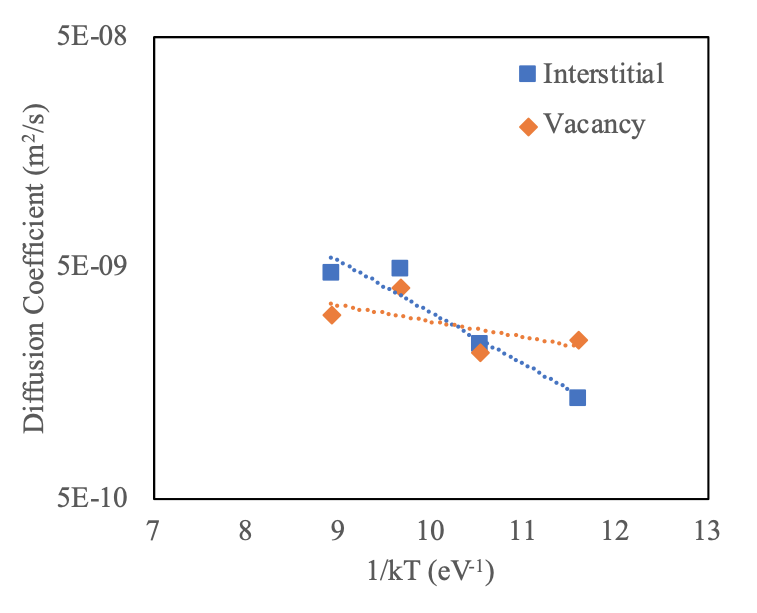
\includegraphics[width=0.75\textwidth]{diff.png} 
 \caption{The vacancy and interstitial diffusion coefficient for $\gamma$-U from 1000 K to 1400 K. Exponential fits to the individual data sets are included as dashed lines.}
 \label{fig:diff}
\end{figure}

\FloatBarrier

\begin{table}[h]
\caption{The migration barrier (E$_m$) for vacancies and interstitials, the activation energy (Q$_A$) for self-diffusion and associated pre-factors in $\gamma$-U over the temperature range of 1000 K - 1400 K.}  \label{tab:diff}
\begin{center}
\begin{tabular}{|c|c|c|}
	\hline
	 & E$_m$ or Q$_A$ (eV) & D$_0$ (m$^2$/s) \\
	 \hline
	 D$_{vac}$ & 0.16 & 1.43x10$^{-8}$ \\
	 D$_{int}$ & 0.52 & 5.56x10$^{-7}$ \\
	 D$_{self}$ & 1.11 & 5.57x10$^{-7}$ \\
	 \hline
\end{tabular}
\end{center}
\label{default}
\end{table}

In order to calculate a self-diffusion coefficient, an average defect formation energy is utilized (averaged from the data in Table \ref{tab:defs} from 1000 K - 1400 K) for both a vacancy (1.7 eV) and an interstitial (0.6 eV). This is a simplification intended to acknowledge the lack of point defect entropies. Ideally, both temperature dependent point defect formation energies and entropies should be utilized. These formation energies are utilized in equation \ref{eqn:selfd}:

\begin{equation}
\label{eqn:selfd}
D_{self} = D_{int}c_{int} + D_{vac}c_{vac}
\end{equation} 

where D$_{int}$ and D$_{vac}$ are the diffusion coefficients from Table \ref{tab:diff} and c$_{int}$ and c$_{vac}$ are the interstitial and vacancy concentrations taken from \textit{exp}$(-E_{def}/kT)$, where $E_{def}$ is either the interstitial or vacancy formation energy averaged from Table \ref{tab:defs}. The entropic contribution on the defect concentration is assumed to be small and thus treated as a factor of one, given that there is no data on the entropic effects of point defects in $\gamma$-U. The calculated self-diffusion coefficient is displayed in Fig. \ref{fig:selfdiff}. Two experimental results are provided as a comparison \cite{rothman1959,adda1959}. Very little other experimental data is available for comparison and none after 1960, as such further experimental studies are warranted. It can be seen that this work slightly over-predicts the self-diffusion in $\gamma$-U compared to the existing experimental results by approximately one order of magnitude. The self-diffusion coefficient is effectively solely due to interstitial diffusion, in that interstitial self-diffusion is approximately four orders of magnitude faster than vacancy diffusion. This is due to the much lower interstitial formation energy, despite the similar diffusion coefficients observed from Fig. \ref{fig:diff}. The activation energy (Q$_A$) from the experimental results are 1.19 eV \cite{adda1959} and 1.15 eV \cite{rothman1959}, while this AIMD work predicts an Q$_A$ of 1.11 eV. This is considered surprisingly excellent agreement. The pre-exponential factors show an over-prediction, where the experimental results are 1.80E-7 \cite{adda1959} and 1.12E-7 \cite{rothman1959}, while the AIMD work is 5.57E-7 (all units in m$^2$/s). However, given the expected inaccuracies in the AIMD simulations due to short times and limited sample size, the omission of actual defect entropies, and the inherent differences in experimental samples and ideal simulation environments, this is quite good agreement and provides confidence in both the modeling methodology and the experimental results. The activation energy and pre-factor for self-diffusion are included in Table \ref{tab:diff}.

 \begin{figure}[h]
 \centering
 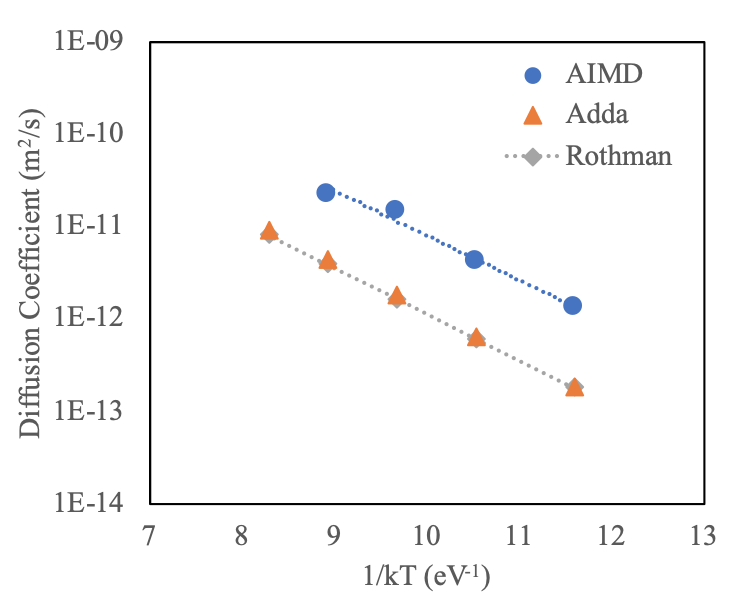
\includegraphics[width=0.75\textwidth]{self_diff.png} 
 \caption{The self-diffusion coefficient for $\gamma$-U from 1000 K to 1400 K. Results are compared to experiments from Rothman \cite{rothman1959} and Adda \cite{adda1959}. }
 \label{fig:selfdiff}
\end{figure}

\FloatBarrier

\section{Conclusions}

In this study, AIMD simulations were performed to calculate the energy as a function of volume for the $\gamma$ phase of U from 800 K to 1400 K. Utilizing the equilibrium volume at each temperature, the bulk modulus, the radial distribution function, the interstitial and vacancy formation energies, and the diffusion coefficients were determined. The lattice constant and thermal expansion are slightly underestimated compared to experiment, while the bulk modulus compares very favorably. Softening of the bulk modulus is observed with increasing temperature, as would be expected. The calculated vacancy formation energies agree with both the experimental results and the previous computational studies. Point defect formation energies increase with increasing temperature, as has been reported in Zr and Al. The vacancy and interstitial diffusion coefficients, as well as the self-diffusion coefficient were calculated. The activation energy compares very favorably to experimentally reported results, while the pre-exponential factor is slightly overestimated, but does show reasonable agreement. The magnitudes of the point defect formation energies in addition to the self-diffusion coefficients are consistent with the notion of self-diffusion via an interstitialcy mechanism in $\gamma$-U. 

This work has served to confirm the findings of previous studies regarding point defects in $\gamma$-U and provides further justification for describing self-diffusion in $\gamma$-U via an interstitialcy mechanism. This was the first \textit{ab initio} molecular dynamics study of point defects in $\gamma$-U and provides the foundation for expansion of computational studies at non-zero temperature in metallic U. 

\section{Acknowledgement}
This work is supported by the U.S. Department of Energy, Office of Nuclear Energy, Nuclear Energy Advanced Modeling and Simulation (NEAMS) Program. This manuscript has been authored by Battelle Energy Alliance, LLC under Contract No. DEAC07-05ID14517 with the U.S. Department of Energy. The United States Government retains and the publisher, by accepting the article for publication, acknowledges that the United States Government retains a nonexclusive, paid-up, irrevocable, world-wide license to publish or reproduce the published form of this manuscript, or allow others to do so, for United States Government purposes.  Los Alamos National Laboratory, an affirmative action/equal opportunity employer, is operated by Los Alamos National Security, LLC, for the National Nuclear Security Administration of the U.S. Department of Energy under Contract No. DE-AC52-06NA25396.  This research made use of the resources of the High Performance Computing Center at Idaho National Laboratory, which is supported by the Office of Nuclear Energy of the U.S. Department of Energy and the Nuclear Science User Facilities under Contract No. DE-AC07-05ID14517.

\section{Data Availability}

The raw/processed data required to reproduce these findings cannot be shared at this time as the data also forms part of an ongoing study.

\section{References}

\bibliography{MARMOTbib}

\end{document} 
